\chapter{Probabilités conditionnelles et indépendance}

\section{Rappels de probabilités}

\subsection{Vocabulaire et loi de probabilité}

\begin{defin}
	Dans le cadre de l'étude des probabilités :

	\begin{itemize}
		\item Une \textbf{expérience aléatoire} est une épreuve dont le résultat dépend du hasard et ne peut pas être prédit avec certitude avant qu'elle ne soit réalisée.
		\item Une \textbf{issue} est un résultat possible de l'expérience aléatoire.
		\item L'\textbf{univers}, noté $\Omega$, est l'ensemble de toutes les issues possibles de cette expérience.
		\item Un \textbf{événement} est une partie de l'univers, c'est-à-dire un ensemble constitué d'une ou de plusieurs issues.
	\end{itemize}
\end{defin}

\begin{ex}
	On lance un dé équilibré à 6 faces :

	\begin{itemize}
		\item L'\textbf{expérience aléatoire} est le lancer du dé.
		\item Une \textbf{issue} est l'obtention d'un nombre (par exemple le $\epsdice{3}$).
		\item L'\textbf{univers} est l'ensemble de tous les résultats possibles : $\Omega = \brac{\epsdice{1}\,;\,\epsdice{2}\,;\,\epsdice{3}\,;\,\epsdice{4}\,;\,\epsdice{5}\,;\,\epsdice{6}}$.
		\item Un \textbf{événement} est par exemple $A$ : \og obtenir un nombre pair \fg{}, ce qui correspond à la partie $\brac{\epsdice{2}\,;\,\epsdice{4}\,;\,\epsdice{6}}$.
	\end{itemize}
\end{ex}

\begin{defin}
	La \textbf{probabilité d'une issue} est la valeur vers laquelle se stabilise la fréquence de réalisation de cette issue lorsqu'on répète l'expérience aléatoire un très grand nombre de fois.

	Soit une expérience aléatoire dont l'univers est $\Omega = \brac{e_1\,;\,e_2\,;\,\dots\,;\,e_n}$.

	Définir une \textbf{loi de probabilité}, c'est associer à chaque issue $e_i$ un nombre réel $p_i$, appelé probabilité de l'issue, tel que :

	\begin{itemize}
		\item $0 \leq p_i \leq 1$ pour chaque issue $e_i$ ;
		\item la somme de toutes les probabilités est égale à $1$ : $\quad p_1 + p_2 + \dots + p_n = 1$.
	\end{itemize}
\end{defin}

\begin{rem}
	Une loi de probabilité est généralement présentée sous la forme d'un tableau :

	\begin{center}
		\rnc{\arraystretch}{1.3}
		\begin{tabular}{|c|c|c|c|c|} \hline
			\ccg\textbf{Issue} $e_i$       & $e_1$ & $e_2$ & $\dots$ & $e_n$ \\ \hline
			\ccg\textbf{Probabilité} $p_i$ & $p_1$ & $p_2$ & $\dots$ & $p_n$ \\ \hline
		\end{tabular}
	\end{center}
\end{rem}

\begin{ex}
	Une classe de $30$ élèves comprend $18$ filles et $12$ garçons.

	On choisit un élève au hasard et l'univers de cette expérience aléatoire est $\Omega = \brac{\text{Fille}\,;\,\text{Garçon}}$.

	\begin{center}
		\rnc{\arraystretch}{1.5}
		\begin{tabular}{|c|c|c|} \hline
			\ccg\textbf{Issue} $e_i$                             & Fille                    & Garçon                   \\ \hline
			\ccg\rule[-4mm]{0mm}{11mm}\textbf{Probabilité} $p_i$ & $\dfrac{18}{30} = 0{,}6$ & $\dfrac{12}{30} = 0{,}4$ \\ \hline
		\end{tabular}
	\end{center}

	On vérifie bien que la somme des probabilités est égale à $1$ : $0{,}6 + 0{,}4 = 1$.
\end{ex}

\begin{defn}
	Soit $A$ un ensemble (ou un événement). Le \textbf{cardinal} de $A$, noté $\card{A}$, correspond au \textbf{nombre d'éléments} qu'il contient.
\end{defn}

\begin{prop}
	Lorsque toutes les issues d'une expérience aléatoire ont la même probabilité, on dit qu'il y a \textbf{équiprobabilité}.

	Pour tout événement $A$ :
	\[
		\p{A} = \dfrac{\card{A}}{\card{\Omega}} = \dfrac{\text{nombre d'issues favorables}}{\text{nombre d'issues possibles}}
	\]
\end{prop}

\begin{prop}
	Soit $A$ un événement d'une expérience aléatoire.

	Si $A$ est constitué des issues $e_1, e_2, \dots, e_k$, alors la probabilité de l'événement $A$ est la somme des probabilités des issues qui le réalisent :
	\[
		\p{A} = \p{e_1} + \p{e_2} + \dots + \p{e_k}
	\]
\end{prop}

\begin{rem}
	Par convention, la probabilité de l'événement impossible, noté $\emptyset$, est égale à $0$.
\end{rem}

\begin{prop}
	Soit une expérience aléatoire d'univers $\Omega$.

	\begin{itemize}
		\item La probabilité de l'univers est $\p{\Omega} = 1$.
		\item Pour tout événement $A$, la probabilité de l'événement contraire $\bar{A}$ est :
		      \[
			      \p{\bar{A}} = 1 - \p{A}
		      \]
	\end{itemize}
\end{prop}

\begin{ex}
	On lance un dé équilibré à 6 faces. Toutes les issues ont la même probabilité $\frac{1}{6}$.

	Soit $E$ l'événement \og obtenir un nombre strictement supérieur à 4 \fg{} $\Rarr E = \brac{\epsdice{5}\,;\,\epsdice{6}}$.
	\[
		\p{E} = \p{\epsdice{5}} + \p{\epsdice{6}} = \dfrac{1}{6} + \dfrac{1}{6} = \dfrac{2}{6} = \dfrac{1}{3}
	\]

	L'événement contraire $\bar{E}$ est \og obtenir un nombre inférieur ou égal à 4 \fg{} $\Rarr \bar{E} = \brac{\epsdice{1}\,;\,\epsdice{2}\,;\,\epsdice{3}\,;\,\epsdice{4}}$.
	\[
		\p{\bar{E}} = 1 - \p{E} = 1 - \dfrac{1}{3} = \dfrac{2}{3}
	\]
\end{ex}

\subsection{Opérations sur les événements}

\begin{defin}
	Soient $A$ et $B$ deux événements d'un même univers $\Omega$.

	\begin{itemize}
		\item L'\textbf{événement contraire} de $A$, noté $\bar{A}$, est constitué de toutes les issues de $\Omega$ qui ne réalisent pas $A$.
		\item L'\textbf{intersection} de $A$ et $B$, notée $A \cap B$ (\og $A$ et $B$ \fg{}), est constituée des issues qui réalisent \textbf{à la fois} $A$ \textbf{et} $B$.
		\item La \textbf{réunion} de $A$ et $B$, notée $A \cup B$ (\og $A$ ou $B$ \fg{}), est constituée des issues qui réalisent $A$, $B$, \textbf{ou les deux en même temps}.
		\item Les événements $A$ et $B$ sont \textbf{incompatibles} si $A \cap B = \emptyset$.
	\end{itemize}
\end{defin}

\begin{center}
	\begin{tikzpicture}
		% Intersection
		\begin{scope}[shift={(0,0)}]
			\draw[gris, thick, rounded corners=4pt] (0,0) rectangle (3.6,2.4);
			\begin{scope}
				\clip (1.35,1.2) circle (0.8);
				\fill[bleu!30] (2.25,1.2) circle (0.8);
			\end{scope}
			\draw[thick, bleu] (1.35,1.2) circle (0.8);
			\draw[thick, rouge] (2.25,1.2) circle (0.8);
			\node at (0.9,1.2) {$A$};
			\node at (2.7,1.2) {$B$};
			\node[font=\small] at (0.25,2.1) {$\Omega$};
			\node[below] at (1.8,-0.05) {$A \cap B$};
		\end{scope}
		% Réunion
		\begin{scope}[shift={(4.4,0)}]
			\draw[gris, thick, rounded corners=4pt] (0,0) rectangle (3.6,2.4);
			\fill[bleu!30] (1.35,1.2) circle (0.8);
			\fill[bleu!30] (2.25,1.2) circle (0.8);
			\draw[thick, bleu] (1.35,1.2) circle (0.8);
			\draw[thick, rouge] (2.25,1.2) circle (0.8);
			\node at (0.9,1.2) {$A$};
			\node at (2.7,1.2) {$B$};
			\node[font=\small] at (0.25,2.1) {$\Omega$};
			\node[below] at (1.8,-0.05) {$A \cup B$};
		\end{scope}
		% Contraire
		\begin{scope}[shift={(8.8,0)}]
			\fill[bleu!30, rounded corners=4pt] (0,0) rectangle (3.6,2.4);
			\fill[white] (1.8,1.2) circle (0.8);
			\draw[gris, thick, rounded corners=4pt] (0,0) rectangle (3.6,2.4);
			\draw[thick, bleu] (1.8,1.2) circle (0.8);
			\node at (1.8,1.2) {$A$};
			\node at (0.45,0.45) {$\bar{A}$};
			\node[font=\small] at (0.25,2.1) {$\Omega$};
			\node[below] at (1.8,-0.05) {$\bar{A}$};
		\end{scope}
	\end{tikzpicture}
\end{center}

\begin{ex}
	On lance un dé équilibré à 6 faces et on considère les événements :

	\begin{itemize}
		\item $E$ : \og obtenir un nombre pair \fg{}, $\quad E = \brac{\epsdice{2}\,;\,\epsdice{4}\,;\,\epsdice{6}}$ ;
		\item $F$ : \og obtenir au plus $4$ \fg{}, $\quad F = \brac{\epsdice{1}\,;\,\epsdice{2}\,;\,\epsdice{3}\,;\,\epsdice{4}}$.
	\end{itemize}

	\begin{enumerate}
		\item L'événement $E \cap F$ : \og obtenir un nombre pair \textbf{et} au plus $4$ \fg{}.

		      Les issues qui réalisent à la fois $E$ et $F$ sont $\epsdice{2}$ et $\epsdice{4}$, donc $E \cap F = \brac{\epsdice{2}\,;\,\epsdice{4}}$ et :
		      \[
			      \p{E \cap F} = \dfrac{2}{6} = \dfrac{1}{3}
		      \]
		\item L'événement $E \cup F$ : \og obtenir un nombre pair \textbf{ou} au plus $4$ \fg{}.

		      Il rassemble les issues qui réalisent $E$, $F$, ou les deux : $E \cup F = \brac{\epsdice{1}\,;\,\epsdice{2}\,;\,\epsdice{3}\,;\,\epsdice{4}\,;\,\epsdice{6}}$ et :
		      \[
			      \p{E \cup F} = \dfrac{5}{6} \approx 0{,}833
		      \]
	\end{enumerate}
\end{ex}

\begin{prop}
	Pour tous événements $A$ et $B$ d'une même expérience aléatoire :
	\[
		\p{A \cup B} = \p{A} + \p{B} - \p{A \cap B}
	\]
	En particulier, si $A$ et $B$ sont incompatibles, alors $\p{A \cup B} = \p{A} + \p{B}$.
\end{prop}

\begin{rem}
	Les issues de $A \cap B$ sont comptées à la fois dans $\p{A}$ et dans $\p{B}$ : il faut donc les retrancher une fois.

	Dans l'exemple précédent : $\p{E \cup F} = \dfrac{3}{6} + \dfrac{4}{6} - \dfrac{2}{6} = \dfrac{5}{6}$.
\end{rem}

\begin{ex}
	\nline
	\begin{wrapstuff}[r]
		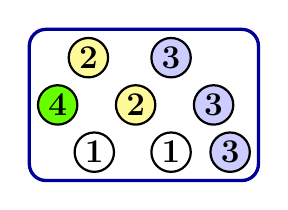
\begin{tikzpicture}[scale=0.3,
				ball/.style={circle, draw=black, thick, text=black, font=\bfseries\large, minimum size=0.5cm, inner sep=0pt},
				ball1/.style={ball, fill=white},
				ball2/.style={ball, fill=yellow!40},
				ball3/.style={ball, fill=blue!20},
				ball4/.style={ball, fill=green!60!yellow}
			]
			\draw[blue!60!black, very thick, rounded corners=6pt] (-1, -0.7) rectangle (8.7, 5.7);
			\node[ball2] at (1.5, 4.5) {2};
			\node[ball3] at (5.0, 4.5) {3};
			\node[ball4] at (0.2, 2.5) {4};
			\node[ball2] at (3.5, 2.5) {2};
			\node[ball3] at (6.8, 2.5) {3};
			\node[ball1] at (1.75, 0.5) {1};
			\node[ball1] at (5.0, 0.5) {1};
			\node[ball3] at (7.5, 0.5) {3};
		\end{tikzpicture}
	\end{wrapstuff}

	On tire au hasard une boule dans l'urne ci-dessous et on note son numéro.

	L'univers de cette expérience aléatoire est :
	\[
		\Omega = \brac{1\,;\,2\,;\,3\,;\,4}
	\]

	Les issues ne sont pas équiprobables : la loi de probabilité est donnée par le tableau suivant.

	\begin{center}
		\rnc{\arraystretch}{1.4}
		\begin{tabular}{|c|c|c|c|c|} \hline
			\ccg\textbf{Issue}                             & $1$            & $2$            & $3$            & $4$            \\ \hline
			\ccg\rule[-4mm]{0mm}{11mm}\textbf{Probabilité} & $\dfrac{2}{8}$ & $\dfrac{2}{8}$ & $\dfrac{3}{8}$ & $\dfrac{1}{8}$ \\ \hline
		\end{tabular}
	\end{center}

	On définit les événements $A = \brac{1\,;\,2}$ et $C = \brac{1\,;\,3}$.

	\begin{itemize}
		\item \textbf{Probabilités de $A$ et de $C$ :}
		      \[
			      \p{A} = \dfrac{2}{8} + \dfrac{2}{8} = \dfrac{4}{8} = 0{,}5 \quad\text{et}\quad \p{C} = \dfrac{2}{8} + \dfrac{3}{8} = \dfrac{5}{8} = 0{,}625
		      \]
		\item \textbf{Événement contraire $\bar{A}$ :}
		      \[
			      \bar{A} = \brac{3\,;\,4} \quad\text{donc}\quad \p{\bar{A}} = \dfrac{4}{8} = 0{,}5
		      \]
		\item \textbf{Intersection $A \cap C$ :}
		      \[
			      A \cap C = \brac{1} \quad\text{donc}\quad \p{A \cap C} = \dfrac{2}{8} = 0{,}25
		      \]
		\item \textbf{Réunion $A \cup C$ :}
		      \[
			      A \cup C = \brac{1\,;\,2\,;\,3} \quad\text{donc}\quad \p{A \cup C} = \dfrac{7}{8} = 0{,}875
		      \]
		      On retrouve ce résultat avec la formule : $\p{A \cup C} = \dfrac{4}{8} + \dfrac{5}{8} - \dfrac{2}{8} = \dfrac{7}{8}$.
	\end{itemize}

	Ces événements se représentent par des diagrammes de Venn :

	\begin{center}
		\begin{tikzpicture}[scale=0.9, dot/.style={circle, fill=black, inner sep=1.2pt}]
			\begin{scope}[shift={(0,0)}]
				\draw[gris, thick, fill=grisLeger, rounded corners=8pt] (0,0) rectangle (6,4);
				\node[anchor=north west] at (0.1, 3.9) {\Large $\Omega$};
				\draw[bleu, thick, fill=bleu!25, fill opacity=0.8] (2.2, 1.6) ellipse (1.8cm and 1.1cm);
				\node at (1.5, 2.2) {\Large $A$};
				\node at (5.0, 2.7) {\Large $\bar{A}$};
				\node[dot, label=right:{$1$}] at (2.9, 1.2) {};
				\node[dot, label=right:{$2$}] at (1.2, 1.1) {};
				\node[dot, label=right:{$3$}] at (4.5, 1.3) {};
				\node[dot, label=right:{$4$}] at (3.0, 3.4) {};
			\end{scope}
			\begin{scope}[shift={(8,0)}]
				\draw[gris, thick, fill=grisLeger, rounded corners=8pt] (0,0) rectangle (6,4);
				\node[anchor=north west] at (0.1, 3.9) {\Large $\Omega$};
				\draw[bleu, thick, fill=bleu!25, fill opacity=0.7] (2.0, 1.6) ellipse (1.7cm and 1.1cm);
				\draw[rouge, thick, fill=rouge!25, fill opacity=0.5] (3.8, 1.8) ellipse (1.7cm and 1.1cm);
				\node at (1.5, 2.2) {\Large $A$};
				\node at (4.6, 2.1) {\Large $C$};
				\node at (2.9, 1.9) {$A \cap C$};
				\node[dot, label=right:{$1$}] at (2.9, 1.2) {};
				\node[dot, label=right:{$2$}] at (1.1, 1.1) {};
				\node[dot, label=right:{$3$}] at (4.5, 1.3) {};
				\node[dot, label=right:{$4$}] at (3.0, 3.4) {};
			\end{scope}
		\end{tikzpicture}
	\end{center}
\end{ex}

\section{Probabilité conditionnelle}

\subsection{Définition et premières propriétés}

\begin{defin}
	Soient $A$ et $B$ deux événements d'un même univers $\Omega$, avec $\p{A} \neq 0$.

	On appelle \textbf{probabilité conditionnelle} de l'événement $B$ sachant l'événement $A$, notée $\pc{A}{B}$, la probabilité que $B$ se réalise sachant que $A$ est réalisé.

	Elle est définie par :
	\[
		\pc{A}{B} = \dfrac{\p{A \cap B}}{\p{A}}
	\]
\end{defin}

\begin{rem}
	\nline
	\begin{center}
		\begin{tikzpicture}[scale=0.5, label_style/.style={font=\small\bfseries}]
			\node (proba) at (0,0) {\LARGE $\pc{\textcolor{rouge}{A}}{\textcolor{vert}{B}}$};
			\draw[<-, ultra thick, vert] (0.7, 0.6) -- (0.5, 1.5) node[left, label_style, text=vert] {Probabilité de $B$\ldots};
			\draw[<-, ultra thick, rouge] (-0.5, -0.6) -- (-0.4, -1.5) node[right, label_style, text=rouge] {\ldots sachant que $A$ est réalisé};
		\end{tikzpicture}
	\end{center}
\end{rem}

\begin{rem}
	Sachant que $A$ est réalisé, l'univers se réduit à $A$ : la probabilité conditionnelle $\pc{A}{B}$ compare la partie de $B$ située dans $A$, c'est-à-dire $A \cap B$, à l'événement $A$ tout entier.

	\begin{center}
		\begin{tikzpicture}
			\draw[gris, thick, rounded corners=4pt] (0,0) rectangle (5,3);
			\node[font=\small] at (0.25,2.7) {$\Omega$};
			\fill[bleu!15] (1.9,1.5) circle (1);
			\begin{scope}
				\clip (1.9,1.5) circle (1);
				\fill[vert!35] (3.1,1.5) circle (1);
			\end{scope}
			\draw[thick, bleu] (1.9,1.5) circle (1);
			\draw[thick, vert] (3.1,1.5) circle (1);
			\node at (1.3,1.5) {$A$};
			\node at (3.7,1.5) {$B$};
			\node[font=\footnotesize] at (2.5,1.5) {$A \cap B$};
		\end{tikzpicture}
	\end{center}
\end{rem}

\begin{ex}
	On lance un dé équilibré à 6 faces.

	On considère les événements $A$ : \og obtenir un nombre pair \fg{} et $B$ : \og obtenir un multiple de $3$ \fg{}.

	On a $A = \brac{\epsdice{2}\,;\,\epsdice{4}\,;\,\epsdice{6}}$, $B = \brac{\epsdice{3}\,;\,\epsdice{6}}$ et $A \cap B = \brac{\epsdice{6}}$, donc :
	\[
		\p{A} = \dfrac{1}{2}, \quad \p{B} = \dfrac{1}{3}, \quad \p{A \cap B} = \dfrac{1}{6}
	\]

	Sachant que le résultat est pair, la probabilité d'obtenir un multiple de $3$ est :
	\[
		\pc{A}{B} = \dfrac{\p{A \cap B}}{\p{A}} = \dfrac{\frac{1}{6}}{\frac{1}{2}} = \dfrac{1}{3}
	\]

	Sachant que le résultat est un multiple de $3$, la probabilité d'obtenir un nombre pair est :
	\[
		\pc{B}{A} = \dfrac{\p{A \cap B}}{\p{B}} = \dfrac{\frac{1}{6}}{\frac{1}{3}} = \dfrac{1}{2}
	\]
\end{ex}

\begin{piege}
	Ne pas confondre $\pc{A}{B}$ et $\pc{B}{A}$ : ces deux probabilités sont en général différentes, comme le montre l'exemple précédent.

	De même, $\pc{A}{B}$ (probabilité de $B$ dans l'univers réduit à $A$) est à distinguer de $\p{A \cap B}$ (probabilité de $A$ et $B$ dans l'univers $\Omega$ tout entier).
\end{piege}

\begin{remarque}[Traduire une phrase en langage probabiliste]
	\nline
	\begin{center}
		\rnc{\arraystretch}{1.4}
		\begin{tabular}{|l|c|} \hline
			\textbf{Expression en français}                                         & \textbf{Notation} \\ \hline
			\og la probabilité de $A$ et de $B$ \fg{}                               & $\p{A \cap B}$    \\ \hline
			\og la probabilité de $A$ ou de $B$ \fg{}                               & $\p{A \cup B}$    \\ \hline
			\og la probabilité de $B$ sachant $A$ \fg{}, \og si $A$ alors $B$ \fg{} & $\pc{A}{B}$       \\ \hline
			\og la probabilité de ne pas avoir $A$ \fg{}                            & $\p{\bar{A}}$     \\ \hline
		\end{tabular}
	\end{center}
\end{remarque}

\begin{prop}
	En situation d'\textbf{équiprobabilité}, pour tous événements $A$ et $B$ avec $A \neq \emptyset$ :
	\[
		\pc{A}{B} = \dfrac{\card{A \cap B}}{\card{A}}
	\]
\end{prop}

\begin{demo}
	En situation d'équiprobabilité, $\p{A \cap B} = \dfrac{\card{A \cap B}}{\card{\Omega}}$ et $\p{A} = \dfrac{\card{A}}{\card{\Omega}}$.

	Donc :
	\[
		\def\arraystretch{2}
		\begin{array}{rcl}
			\pc{A}{B} & = & \dfrac{\p{A \cap B}}{\p{A}}                                                                                       \\
			          & = & \dfrac{\card{A \cap B}}{\card{\Omega}} \times \dfrac{\card{\Omega}}{\card{A}} = \dfrac{\card{A \cap B}}{\card{A}}
		\end{array}
	\]
\end{demo}

\begin{prop}
	Soient $A$ et $B$ deux événements avec $\p{A} \neq 0$.

	\begin{itemize}
		\item $0 \leq \pc{A}{B} \leq 1$ ;
		\item $\pc{A}{\bar{B}} = 1 - \pc{A}{B}$ ;
		\item \textbf{règle du produit :} $\p{A \cap B} = \p{A} \times \pc{A}{B}$.
	\end{itemize}
\end{prop}

\begin{demo}
	\nline
	\begin{itemize}
		\item Les issues de $A \cap B$ sont aussi des issues de $A$, donc $0 \leq \p{A \cap B} \leq \p{A}$.

		      En divisant par $\p{A} > 0$, on obtient $0 \leq \pc{A}{B} \leq 1$.
		\item Les événements $A \cap B$ et $A \cap \bar{B}$ sont incompatibles et leur réunion est $A$, donc :
		      \[
			      \p{A} = \p{A \cap B} + \p{A \cap \bar{B}}
		      \]

		      En divisant par $\p{A}$, on obtient $1 = \pc{A}{B} + \pc{A}{\bar{B}}$.
		\item La règle du produit s'obtient en multipliant par $\p{A}$ la définition $\pc{A}{B} = \dfrac{\p{A \cap B}}{\p{A}}$.
	\end{itemize}
\end{demo}

\newpage

\subsection{Calcul à l'aide d'un tableau croisé}

\begin{methode}[Calculer des probabilités conditionnelles à l'aide d'un tableau croisé]
	Une étude pharmaceutique est réalisée sur un échantillon de $800$ patients afin d'évaluer l'efficacité de deux médicaments.

	Chaque patient a pris exactement l'un des deux médicaments.

	Les résultats sont résumés dans le tableau croisé d'effectifs ci-dessous :

	\begin{center}
		\rnc{\arraystretch}{1.3}
		\begin{tabular}{|c|c|c|c|} \hline
			~                           & \ccg{Médicament A} & \ccg{Médicament B} & \ccg\textbf{Total} \\ \hline
			\ccg{Guéri ($G$)}           & $383$              & $291$              & $674$              \\ \hline
			\ccg{Non guéri ($\bar{G}$)} & $72$               & $54$               & $126$              \\ \hline
			\ccg\textbf{Total}          & $455$              & $345$              & $800$              \\ \hline
		\end{tabular}
	\end{center}

	On choisit un patient au hasard.

	On note $A$ : \og le patient a pris le médicament A \fg{}, $B$ : \og le patient a pris le médicament B \fg{} (donc $B = \bar{A}$) et $G$ : \og le patient est guéri \fg{}.

	\begin{enumerate}
		\item Calculer la probabilité que le patient ait pris le médicament A sachant qu'il est guéri.
		\item Calculer la probabilité que le patient soit guéri sachant qu'il a pris le médicament B.
		\item Calculer $\p{A \cap G}$, $\pc{A}{G}$ et $\pc{G}{A}$, puis comparer ces trois valeurs.
	\end{enumerate}

	\begin{correction}
		\nline
		\begin{enumerate}
			\item On cherche $\pc{G}{A}$.

			      La condition est $G$ : on se restreint à la ligne des patients guéris ($674$ personnes), parmi lesquelles $383$ ont pris le médicament A.
			      \[
				      \pc{G}{A} = \dfrac{\card{G \cap A}}{\card{G}} = \dfrac{383}{674} \approx 0{,}568
			      \]
			\item On cherche $\pc{B}{G}$.

			      La condition est $B$ : on se restreint à la colonne du médicament B ($345$ personnes), parmi lesquelles $291$ sont guéries.
			      \[
				      \pc{B}{G} = \dfrac{\card{B \cap G}}{\card{B}} = \dfrac{291}{345} \approx 0{,}843
			      \]
			\item Les trois quantités se lisent dans la même case du tableau ($383$ patients), mais ne se rapportent pas au même effectif total :
			      \[
				      \p{A \cap G} = \dfrac{383}{800} \approx 0{,}479 \qquad \pc{A}{G} = \dfrac{383}{455} \approx 0{,}842 \qquad \pc{G}{A} = \dfrac{383}{674} \approx 0{,}568
			      \]
			      \begin{itemize}
				      \item $\p{A \cap G}$ : on rapporte à l'effectif total ($800$) ;
				      \item $\pc{A}{G}$ : on rapporte à l'effectif de la colonne du médicament A ($455$) ;
				      \item $\pc{G}{A}$ : on rapporte à l'effectif de la ligne des guéris ($674$).
			      \end{itemize}
		\end{enumerate}
	\end{correction}
\end{methode}

\newpage

\section{Arbres pondérés et probabilités totales}

\subsection{Règles de construction d'un arbre pondéré}

Un arbre pondéré (ou arbre de probabilités) permet de représenter la succession de plusieurs événements.

Sur chaque branche, on inscrit la probabilité (éventuellement conditionnelle) de l'événement situé à son extrémité.

\begin{center}
	\begin{tikzpicture}[scale=1.2, >=Stealth, thick]
		\node (root) at (0,0) {};
		\node (A) at (2.5,1) {$A$};
		\node (Abar) at (2.5,-1) {$\bar{A}$};
		\node (AB) at (5.5,1.5) {$B$};
		\node (ABbar) at (5.5,0.5) {$\bar{B}$};
		\node (AbarB) at (5.5,-0.5) {$B$};
		\node (AbarBbar) at (5.5,-1.5) {$\bar{B}$};
		\draw[->] (root) -- (A) node[sloped, midway, above] {$\p{A}$};
		\draw[->] (root) -- (Abar) node[sloped, midway, below] {$\p{\bar{A}}$};
		\draw[->] (A) -- (AB) node[sloped, midway, above] {$\pc{A}{B}$};
		\draw[->] (A) -- (ABbar) node[sloped, midway, below] {$\pc{A}{\bar{B}}$};
		\draw[->] (Abar) -- (AbarB) node[sloped, midway, above] {$\pc{\bar{A}}{B}$};
		\draw[->] (Abar) -- (AbarBbar) node[sloped, midway, below] {$\pc{\bar{A}}{\bar{B}}$};
		\node[right] at (5.8,1.5) {$\Rarr A \cap B$};
		\node[right] at (5.8,0.5) {$\Rarr A \cap \bar{B}$};
		\node[right] at (5.8,-0.5) {$\Rarr \bar{A} \cap B$};
		\node[right] at (5.8,-1.5) {$\Rarr \bar{A} \cap \bar{B}$};
	\end{tikzpicture}
\end{center}

\begin{propriete}[Règles de l'arbre pondéré]
	\nline
	\begin{itemize}
		\item \textbf{Règle des n\oe{}uds :} la somme des probabilités des branches issues d'un même nœud est égale à $1$.
		      \[
			      \p{A} + \p{\bar{A}} = 1 \quad \text{et} \quad \pc{A}{B} + \pc{A}{\bar{B}} = 1
		      \]
		\item \textbf{Règle du produit :} la probabilité de l'événement correspondant à un chemin est égale au produit des probabilités portées par les branches de ce chemin.
		      \[
			      \p{A \cap B} = \p{A} \times \pc{A}{B}
		      \]
		      % \item \textbf{Règle de la somme (probabilité totale) :} la probabilité d'un événement est égale à la somme des probabilités des chemins qui le réalisent.
		      %       \[
		      % 	      \p{B} = \p{A \cap B} + \p{\bar{A} \cap B}
		      %       \]
	\end{itemize}
\end{propriete}

\begin{ex}
	Une urne contient $3$ boules blanches et $2$ boules rouges.

	On tire successivement \textbf{sans remise} deux boules de l'urne.

	Pour $i \in \brac{1\,;\,2}$, on note $B_i$ l'événement \og la $i$-ème boule tirée est blanche \fg{} et $R_i = \bar{B_i}$.

	\begin{center}
		\begin{tikzpicture}[scale=1.1, >=Stealth, thick]
			\node (root) at (0,0) {};
			\node (B1) at (2.5,1.2) {$B_1$};
			\node (R1) at (2.5,-1.2) {$R_1$};
			\node (B1B2) at (5.5,1.8) {$B_2$};
			\node (B1R2) at (5.5,0.6) {$R_2$};
			\node (R1B2) at (5.5,-0.6) {$B_2$};
			\node (R1R2) at (5.5,-1.8) {$R_2$};

			\draw[->] (root) -- (B1) node[sloped, midway, above left] {$\frac{3}{5}$};
			\draw[->] (root) -- (R1) node[sloped, midway, below left] {$\frac{2}{5}$};
			\draw[->] (B1) -- (B1B2) node[sloped, midway, above] {$\frac{2}{4}$};
			\draw[->] (B1) -- (B1R2) node[sloped, midway, below] {$\frac{2}{4}$};
			\draw[->] (R1) -- (R1B2) node[sloped, midway, above] {$\frac{3}{4}$};
			\draw[->] (R1) -- (R1R2) node[sloped, midway, below] {$\frac{1}{4}$};

			\node[right] at (5.8,1.8) {$\Rarr \p{B_1 \cap B_2} = \dfrac{3}{5} \times \dfrac{2}{4} = \dfrac{3}{10}$};
			\node[right] at (5.8,0.6) {$\Rarr \p{B_1 \cap R_2} = \dfrac{3}{5} \times \dfrac{2}{4} = \dfrac{3}{10}$};
			\node[right] at (5.8,-0.6) {$\Rarr \p{R_1 \cap B_2} = \dfrac{2}{5} \times \dfrac{3}{4} = \dfrac{3}{10}$};
			\node[right] at (5.8,-1.8) {$\Rarr \p{R_1 \cap R_2} = \dfrac{2}{5} \times \dfrac{1}{4} = \dfrac{1}{10}$};
		\end{tikzpicture}
	\end{center}

	Après un premier tirage d'une boule blanche, il reste $2$ blanches et $2$ rouges, d'où $\pc{B_1}{B_2} = \dfrac{2}{4}$.

	Après un premier tirage d'une boule rouge, il reste $3$ blanches et $1$ rouge, d'où $\pc{R_1}{B_2} = \dfrac{3}{4}$.

	D'après la règle de la somme, la probabilité que la deuxième boule soit blanche est :
	\[
		\p{B_2} = \p{B_1 \cap B_2} + \p{R_1 \cap B_2} = \dfrac{3}{10} + \dfrac{3}{10} = \dfrac{3}{5}
	\]
\end{ex}

\subsection{Partition de l'univers et formule des probabilités totales}

\begin{defin}
	Soient $A_1, A_2, \dots, A_n$ des événements de probabilités non nulles d'un univers $\Omega$.

	On dit que $A_1, A_2, \dots, A_n$ forment une \textbf{partition} de $\Omega$ (ou un système complet d'événements) si :
	\begin{itemize}
		\item les événements sont deux à deux incompatibles : pour tous $i \neq j$, $A_i \cap A_j = \emptyset$ ;
		\item leur réunion est l'univers tout entier : $A_1 \cup A_2 \cup \dots \cup A_n = \Omega$.
	\end{itemize}
\end{defin}

\begin{rem}
	Pour tout événement $A$ tel que $0 < \p{A} < 1$, les événements $A$ et $\bar{A}$ forment une partition de l'univers $\Omega$.
\end{rem}

\begin{theoreme}[Formule des probabilités totales]
	Soient $A_1, A_2, \dots, A_n$ une partition de l'univers $\Omega$.

	Pour tout événement $B$, la probabilité de $B$ est la somme des probabilités des intersections de $B$ avec chaque événement de la partition :
	\[
		\p{B} = \p{A_1 \cap B} + \p{A_2 \cap B} + \dots + \p{A_n \cap B}
	\]
	C'est-à-dire :
	\[
		\p{B} = \p{A_1} \times \pc{A_1}{B} + \p{A_2} \times \pc{A_2}{B} + \dots + \p{A_n} \times \pc{A_n}{B}
	\]
	En particulier, pour une partition $A$ et $\bar{A}$ :
	\[
		\p{B} = \p{A \cap B} + \p{\bar{A} \cap B} = \p{A} \times \pc{A}{B} + \p{\bar{A}} \times \pc{\bar{A}}{B}
	\]
\end{theoreme}

\begin{center}
	\begin{tikzpicture}[scale=0.9]
		\draw[gris, thick, rounded corners=4pt] (0,0) rectangle (6,4);
		\node[above left] at (0,4) {$\Omega$};
		\fill[bleu!20] (3,1.8) ellipse (2.5 and 1.3);
		\draw[gris, thick] (2,0) -- (2,4);
		\draw[gris, thick] (4,0) -- (4,4);
		\draw[bleu, thick] (3,1.8) ellipse (2.5 and 1.3);
		\node at (1,3.6) {$A_1$};
		\node at (3,3.6) {$A_2$};
		\node at (5,3.6) {$A_3$};
		\node[font=\footnotesize] at (1.25,1.8) {$A_1 \cap B$};
		\node[font=\footnotesize] at (3,1.8) {$A_2 \cap B$};
		\node[font=\footnotesize] at (4.75,1.8) {$A_3 \cap B$};
		\node[bleu] at (5.45,2.9) {$B$};
	\end{tikzpicture}
\end{center}

\begin{demo}
	Comme $A_1, A_2, \dots, A_n$ est une partition de $\Omega$, toute issue de $B$ appartient à un et un seul des $A_i$.

	On peut donc décomposer $B$ en une réunion d'événements deux à deux incompatibles :
	\[
		B = (A_1 \cap B) \cup (A_2 \cap B) \cup \dots \cup (A_n \cap B)
	\]
	La probabilité d'une réunion d'événements deux à deux incompatibles est la somme de leurs probabilités :
	\[
		\p{B} = \p{A_1 \cap B} + \p{A_2 \cap B} + \dots + \p{A_n \cap B}
	\]
	En appliquant la règle du produit $\p{A_i \cap B} = \p{A_i} \times \pc{A_i}{B}$ à chaque terme, on obtient la seconde formule.
\end{demo}

\begin{methode}[Appliquer la formule des probabilités totales et inverser le conditionnement]
	Lors d'une épidémie chez des bovins, $2\,\%$ de la population est porteuse d'une maladie $M$.

	On utilise un test de dépistage $T$ qui présente les caractéristiques suivantes :
	\begin{itemize}
		\item si un animal est malade, le test est positif avec une probabilité de $0{,}85$ ;
		\item si un animal est sain, le test est négatif avec une probabilité de $0{,}95$.
	\end{itemize}

	\begin{enumerate}
		\item Représenter la situation par un arbre pondéré.
		\item Calculer la probabilité qu'un animal choisi au hasard ait un test positif.
		\item Si le test d'un bovin est positif, quelle est la probabilité qu'il soit réellement malade ?
	\end{enumerate}

	\begin{correction}
		\nline
		\begin{enumerate}
			\item Construction de l'arbre pondéré.

			      Si l'animal est sain, le test est positif avec la probabilité $1 - 0{,}95 = 0{,}05$.

			      \begin{center}
				      \begin{tikzpicture}[scale=1.1, >=Stealth, thick]
					      \node (root) at (0,0) {};
					      \node (M) at (2.5,1.2) {$M$};
					      \node (Mbar) at (2.5,-1.2) {$\bar{M}$};
					      \node (MT) at (5.5,1.8) {$T$};
					      \node (MTbar) at (5.5,0.6) {$\bar{T}$};
					      \node (MbarT) at (5.5,-0.6) {$T$};
					      \node (MbarTbar) at (5.5,-1.8) {$\bar{T}$};

					      \draw[->] (root) -- (M) node[sloped, midway, above] {$0{,}02$};
					      \draw[->] (root) -- (Mbar) node[sloped, midway, below] {$0{,}98$};
					      \draw[->] (M) -- (MT) node[sloped, midway, above] {$0{,}85$};
					      \draw[->] (M) -- (MTbar) node[sloped, midway, below] {$0{,}15$};
					      \draw[->] (Mbar) -- (MbarT) node[sloped, midway, above] {$0{,}05$};
					      \draw[->] (Mbar) -- (MbarTbar) node[sloped, midway, below] {$0{,}95$};
				      \end{tikzpicture}
			      \end{center}

			\item $M$ et $\bar{M}$ forment une partition de l'univers.

			      D'après la formule des probabilités totales :
			      \[
				      \def\arraystretch{1.3}
				      \begin{array}{rcl}
					      \p{T} & = & \p{M \cap T} + \p{\bar{M} \cap T}                           \\
					            & = & \p{M} \times \pc{M}{T} + \p{\bar{M}} \times \pc{\bar{M}}{T} \\
					            & = & 0{,}02 \times 0{,}85 + 0{,}98 \times 0{,}05                 \\
					            & = & 0{,}017 + 0{,}049 = 0{,}066
				      \end{array}
			      \]
			      La probabilité que le test soit positif est $0{,}066$ (soit $6{,}6\,\%$).

			\item On cherche $\pc{T}{M}$, probabilité \og inverse \fg{} de $\pc{M}{T} = 0{,}85$ :
			      \[
				      \pc{T}{M} = \dfrac{\p{M \cap T}}{\p{T}} = \dfrac{0{,}017}{0{,}066} = \dfrac{17}{66} \approx 0{,}258
			      \]
			      Sachant que le test est positif, l'animal a environ $25{,}8\,\%$ de chances d'être malade.

			      Cette valeur est bien plus faible que $\pc{M}{T} = 0{,}85$ : la maladie étant rare, les faux positifs sont nombreux.
		\end{enumerate}
	\end{correction}
\end{methode}

\section{Indépendance de deux événements}

\subsection{Définition et propriétés}

\begin{defin}
	Deux événements $A$ et $B$ sont dits \textbf{indépendants} si et seulement si :
	\[
		\p{A \cap B} = \p{A} \times \p{B}
	\]
\end{defin}

\begin{prop}
	Si $\p{A} \neq 0$, alors $A$ et $B$ sont indépendants si et seulement si :
	\[
		\pc{A}{B} = \p{B}
	\]

	De même, si $\p{B} \neq 0$, $A$ et $B$ sont indépendants si et seulement si $\pc{B}{A} = \p{A}$.
\end{prop}

\newpage

\begin{demo}
	Supposons $\p{A} \neq 0$.
	\[
		\def\arraystretch{1.8}
		\begin{array}{rcl}
			A \text{ et } B \text{ indépendants} & \eqv & \p{A \cap B} = \p{A} \times \p{B}   \\
			                                     & \eqv & \dfrac{\p{A \cap B}}{\p{A}} = \p{B} \\
			                                     & \eqv & \pc{A}{B} = \p{B}
		\end{array}
	\]

	Le raisonnement est le même en échangeant les rôles de $A$ et $B$.
\end{demo}

\begin{rem}
	Deux événements sont donc indépendants lorsque la réalisation de l'un ne modifie pas la probabilité de l'autre.
\end{rem}

\begin{ex}
	On lance un dé équilibré à 6 faces.

	Soient :
	\begin{itemize}
		\item $A$ : \og obtenir un nombre pair \fg{} avec $\p{A}=\dfrac{1}{2}$.
		\item $B$ : \og obtenir un multiple de $3$ \fg{} avec $\p{B}=\dfrac{1}{3}$.
		\item $A\cap B$ : \og obtenir un nombre pair \textbf{et} multiple de $3$ \fg{}. Donc $A\cap B :\brac{\epsdice{6}}\Rarr\p{A \cap B} = \dfrac{1}{6}$.
	\end{itemize}

	On a :
	\[
		\p{A} \times \p{B} = \dfrac{1}{2} \times \dfrac{1}{3} = \dfrac{1}{6} = \p{A \cap B}
	\]

	Donc les événements $A$ et $B$ sont indépendants.
\end{ex}

\begin{attention}
	Ne pas confondre événements \textbf{indépendants} et événements \textbf{incompatibles} !

	\begin{itemize}
		\item Deux événements $A$ et $B$ sont \textbf{incompatibles} si $A \cap B = \emptyset$, c'est-à-dire $\p{A \cap B} = 0$.
		\item Deux événements de probabilités non nulles ne peuvent pas être à la fois incompatibles et indépendants : s'ils étaient incompatibles, on aurait $\p{A \cap B} = 0$, alors que $\p{A} \times \p{B} \neq 0$.
	\end{itemize}
\end{attention}

\begin{prop}
	Si deux événements $A$ et $B$ sont indépendants, alors les événements $\bar{A}$ et $B$ sont également indépendants.

	Il en est de même pour $A$ et $\bar{B}$, ainsi que pour $\bar{A}$ et $\bar{B}$.
\end{prop}

\begin{demo}
	D'après la formule des probabilités totales appliquée à la partition $A$ et $\bar{A}$, on a $\p{B} = \p{A \cap B} + \p{\bar{A} \cap B}$, donc :
	\[
		\p{\bar{A} \cap B} = \p{B} - \p{A \cap B}
	\]

	Comme $A$ et $B$ sont indépendants, $\p{A \cap B} = \p{A} \times \p{B}$.

	Ainsi :
	\[
		\p{\bar{A} \cap B} = \p{B} - \p{A} \times \p{B} = \pa{1 - \p{A}} \times \p{B} = \p{\bar{A}} \times \p{B}
	\]

	Ce qui prouve que $\bar{A}$ et $B$ sont indépendants.

	En échangeant les rôles de $A$ et $B$, on en déduit que $A$ et $\bar{B}$ sont indépendants.

	En appliquant ce résultat à $\bar{A}$ et $B$, qui sont indépendants, on obtient que $\bar{A}$ et $\bar{B}$ sont indépendants.
\end{demo}

\newpage

\begin{methode}[Démontrer l'indépendance de deux événements]
	On tire une carte au hasard dans un jeu de $32$ cartes.

	On note $R$ l'événement \og on tire un roi \fg{} et $T$ l'événement \og on tire un trèfle \fg{}.

	\begin{enumerate}
		\item Les événements $R$ et $T$ sont-ils indépendants ?
		\item Si l'on ajoute $2$ jokers au jeu de $32$ cartes, les événements $R$ et $T$ restent-ils indépendants ?
	\end{enumerate}

	\begin{correction}
		\nline
		\begin{enumerate}
			\item Dans le jeu de $32$ cartes, il y a $4$ rois, $8$ trèfles et un seul roi de trèfle :
			      \[
				      \p{R} = \dfrac{4}{32} = \dfrac{1}{8}, \quad \p{T} = \dfrac{8}{32} = \dfrac{1}{4}, \quad \p{R \cap T} = \dfrac{1}{32}
			      \]

			      On calcule :
			      \[
				      \p{R} \times \p{T} = \dfrac{1}{8} \times \dfrac{1}{4} = \dfrac{1}{32} = \p{R \cap T}
			      \]

			      Donc les événements $R$ et $T$ sont indépendants.

			\item Avec $34$ cartes (les jokers ne sont ni des rois, ni des trèfles) :
			      \[
				      \p{R} = \dfrac{4}{34} = \dfrac{2}{17}, \quad \p{T} = \dfrac{8}{34} = \dfrac{4}{17}, \quad \p{R \cap T} = \dfrac{1}{34}
			      \]

			      On calcule :
			      \[
				      \p{R} \times \p{T} = \dfrac{2}{17} \times \dfrac{4}{17} = \dfrac{8}{289} \neq \dfrac{1}{34}
			      \]

			      Les événements $R$ et $T$ ne sont plus indépendants.
		\end{enumerate}
	\end{correction}
\end{methode}

\section{Succession d'épreuves indépendantes et schéma de Bernoulli}

\subsection{Succession de deux épreuves indépendantes}

\begin{defin}
	Deux épreuves aléatoires sont dites \textbf{indépendantes} si le résultat de l'une n'a aucune influence sur les probabilités des résultats de l'autre.
\end{defin}

\begin{rem}
	L'indépendance de deux épreuves est une hypothèse de modélisation : elle résulte de l'analyse de la situation (par exemple, un tirage avec remise ou le lancer de deux dés distincts).
\end{rem}

\begin{prop}
	Lors de la succession de deux épreuves indépendantes, si $A$ est un événement de la première épreuve et $B$ un événement de la seconde, alors $A$ et $B$ sont indépendants :
	\[
		\p{A \cap B} = \p{A} \times \p{B} \quad\text{et, si } \p{A} \neq 0, \quad \pc{A}{B} = \p{B}
	\]

	Dans l'arbre pondéré, les probabilités portées par les branches du second niveau sont donc les mêmes quel que soit le résultat de la première épreuve.
\end{prop}

\begin{ex}
	Une urne contient $3$ boules blanches et $2$ boules rouges.

	On tire une boule au hasard, \textbf{avec remise}, puis on effectue un second tirage.

	On note $B_i$ l'événement \og la $i$-ème boule tirée est blanche \fg{} et $R_i = \bar{B_i}$.

	La composition de l'urne est identique à chaque tirage : $\p{B_i} = \dfrac{3}{5} = 0{,}6$ et $\p{R_i} = \dfrac{2}{5} = 0{,}4$.

	\begin{center}
		\begin{tikzpicture}[scale=1.1, >=Stealth, thick]
			\node (root) at (0,0) {};
			\node (B1) at (2.5,1.2) {$B_1$};
			\node (R1) at (2.5,-1.2) {$R_1$};
			\node (B1B2) at (5.5,1.8) {$B_2$};
			\node (B1R2) at (5.5,0.6) {$R_2$};
			\node (R1B2) at (5.5,-0.6) {$B_2$};
			\node (R1R2) at (5.5,-1.8) {$R_2$};

			\draw[->] (root) -- (B1) node[sloped, midway, above] {$0{,}6$};
			\draw[->] (root) -- (R1) node[sloped, midway, below] {$0{,}4$};
			\draw[->] (B1) -- (B1B2) node[sloped, midway, above] {$0{,}6$};
			\draw[->] (B1) -- (B1R2) node[sloped, midway, below] {$0{,}4$};
			\draw[->] (R1) -- (R1B2) node[sloped, midway, above] {$0{,}6$};
			\draw[->] (R1) -- (R1R2) node[sloped, midway, below] {$0{,}4$};

			\node[right] at (5.8,1.8) {$\Rarr \p{B_1 \cap B_2} = 0{,}6 \times 0{,}6 = 0{,}36$};
			\node[right] at (5.8,0.6) {$\Rarr \p{B_1 \cap R_2} = 0{,}6 \times 0{,}4 = 0{,}24$};
			\node[right] at (5.8,-0.6) {$\Rarr \p{R_1 \cap B_2} = 0{,}4 \times 0{,}6 = 0{,}24$};
			\node[right] at (5.8,-1.8) {$\Rarr \p{R_1 \cap R_2} = 0{,}4 \times 0{,}4 = 0{,}16$};
		\end{tikzpicture}
	\end{center}

	On peut aussi représenter la situation par un tableau à double entrée, qui donne la probabilité de chaque intersection :

	\begin{center}
		\rnc{\arraystretch}{1.3}
		\begin{tabular}{|c|c|c|c|} \hline
			~                  & \ccg{$B_2$} & \ccg{$R_2$} & \ccg\textbf{Total} \\ \hline
			\ccg{$B_1$}        & $0{,}36$    & $0{,}24$    & $0{,}6$            \\ \hline
			\ccg{$R_1$}        & $0{,}24$    & $0{,}16$    & $0{,}4$            \\ \hline
			\ccg\textbf{Total} & $0{,}6$     & $0{,}4$     & $1$                \\ \hline
		\end{tabular}
	\end{center}
\end{ex}

\begin{attention}
	Un tirage \textbf{sans remise} ne fournit pas nécessairement deux épreuves indépendantes.

	Si, dans l'urne précédente (contenant 3 boules blanches et 2 rouges), on effectuait un tirage \textbf{sans remise}, la probabilité de tirer une boule blanche au deuxième tirage sachant qu'on a déjà tiré une boule blanche au premier serait $\pc{B_1}{B_2} = \dfrac{2}{4} = 0{,}5$, alors que la probabilité initiale de l'événement $B_2$ reste $\p{B_2} = \dfrac{3}{5} = 0{,}6$.

	Puisque $\pc{B_1}{B_2} \neq \p{B_2}$, les événements $B_1$ et $B_2$ ne sont pas indépendants dans ce cas.
\end{attention}

\subsection{Épreuve et schéma de Bernoulli}

\begin{defin}
	\nline
	\begin{wrapstuff}[r]
		\begin{tikzpicture}[>=Stealth, thick]
			\coordinate (root) at (0,0);
			\node (S) at (2,0.8) {$S$};
			\node (Sbar) at (2,-0.8) {$\bar{S}$};
			\draw[->] (root) -- (S) node[sloped, midway, above] {$p$};
			\draw[->] (root) -- (Sbar) node[sloped, midway, below] {$1-p$};
		\end{tikzpicture}
	\end{wrapstuff}

	Une \textbf{épreuve de Bernoulli} de paramètre $p$ (où $0 < p < 1$) est une expérience aléatoire qui ne comporte que deux issues possibles :

	\begin{itemize}
		\item le \textbf{succès}, noté $S$, de probabilité $\p{S} = p$ ;
		\item l'\textbf{échec}, noté $\bar{S}$, de probabilité $\p{\bar{S}} = 1 - p$.
	\end{itemize}
\end{defin}

\begin{defin}
	Un \textbf{schéma de Bernoulli} de paramètres $n$ et $p$ est la répétition de $n$ épreuves de Bernoulli identiques et indépendantes de paramètre $p$.
\end{defin}

\begin{prop}
	Dans l'arbre représentant un schéma de Bernoulli à $n$ répétitions :
	\begin{itemize}
		\item l'arbre comporte $2^n$ chemins ;
		\item tout chemin comportant $k$ succès et $\pa{n - k}$ échecs a pour probabilité $p^k \times (1 - p)^{n - k}$.
	\end{itemize}
\end{prop}

\begin{rem}
	La seconde propriété résulte de la règle du produit : les épreuves étant indépendantes et identiques, chaque succès contribue pour un facteur $p$ et chaque échec pour un facteur $1 - p$.
\end{rem}

\newpage

\begin{methode}[Calculer une probabilité sur un schéma de Bernoulli]
	Un joueur effectue $3$ tirs indépendants.

	La probabilité de réussir un tir est $p = 0{,}3$.

	On note $S$ l'événement \og réussir le tir \fg{} et $\bar{S}$ l'événement \og manquer le tir \fg{}.

	\begin{enumerate}
		\item Représenter l'expérience par un arbre pondéré.
		\item Calculer la probabilité d'obtenir exactement deux réussites.
		\item Calculer la probabilité d'obtenir au moins une réussite.
	\end{enumerate}

	\begin{correction}
		\nline
		\begin{enumerate}
			\item Arbre pondéré pour $n = 3$ répétitions ($p = 0{,}3$ et $1 - p = 0{,}7$) :

			      \begin{center}
				      \begin{tikzpicture}[scale=0.9, >=Stealth, thick]
					      \node (root) at (0,0) {};
					      \node (S1) at (2.5,2.5) {$S$};
					      \node (E1) at (2.5,-2.5) {$\bar{S}$};
					      \node (S1S2) at (5,3.75) {$S$};
					      \node (S1E2) at (5,1.25) {$\bar{S}$};
					      \node (E1S2) at (5,-1.25) {$S$};
					      \node (E1E2) at (5,-3.75) {$\bar{S}$};
					      \node (SSS) at (7.5,4.375) {$S$};
					      \node (SSE) at (7.5,3.125) {$\bar{S}$};
					      \node (SES) at (7.5,1.875) {$S$};
					      \node (SEE) at (7.5,0.625) {$\bar{S}$};
					      \node (ESS) at (7.5,-0.625) {$S$};
					      \node (ESE) at (7.5,-1.875) {$\bar{S}$};
					      \node (EES) at (7.5,-3.125) {$S$};
					      \node (EEE) at (7.5,-4.375) {$\bar{S}$};
					      \draw[->] (root) -- (S1) node[sloped, midway, above] {$0{,}3$};
					      \draw[->] (root) -- (E1) node[sloped, midway, below] {$0{,}7$};
					      \draw[->] (S1) -- (S1S2) node[sloped, midway, above] {$0{,}3$};
					      \draw[->] (S1) -- (S1E2) node[sloped, midway, below] {$0{,}7$};
					      \draw[->] (E1) -- (E1S2) node[sloped, midway, above] {$0{,}3$};
					      \draw[->] (E1) -- (E1E2) node[sloped, midway, below] {$0{,}7$};
					      \draw[->] (S1S2) -- (SSS) node[sloped, midway, above] {$0{,}3$};
					      \draw[->] (S1S2) -- (SSE) node[sloped, midway, below] {$0{,}7$};
					      \draw[->] (S1E2) -- (SES) node[sloped, midway, above] {$0{,}3$};
					      \draw[->] (S1E2) -- (SEE) node[sloped, midway, below] {$0{,}7$};
					      \draw[->] (E1S2) -- (ESS) node[sloped, midway, above] {$0{,}3$};
					      \draw[->] (E1S2) -- (ESE) node[sloped, midway, below] {$0{,}7$};
					      \draw[->] (E1E2) -- (EES) node[sloped, midway, above] {$0{,}3$};
					      \draw[->] (E1E2) -- (EEE) node[sloped, midway, below] {$0{,}7$};
					      \node[right] at (7.8,4.375) {$\Rarr (S\,;\,S\,;\,S) : 0{,}3^3 = 0{,}027$};
					      \node[right] at (7.8,3.125) {$\Rarr (S\,;\,S\,;\,\bar{S}) : 0{,}3^2 \times 0{,}7 = 0{,}063$};
					      \node[right] at (7.8,1.875) {$\Rarr (S\,;\,\bar{S}\,;\,S) : 0{,}3^2 \times 0{,}7 = 0{,}063$};
					      \node[right] at (7.8,0.625) {$\Rarr (S\,;\,\bar{S}\,;\,\bar{S}) : 0{,}3 \times 0{,}7^2 = 0{,}147$};
					      \node[right] at (7.8,-0.625) {$\Rarr (\bar{S}\,;\,S\,;\,S) : 0{,}3^2 \times 0{,}7 = 0{,}063$};
					      \node[right] at (7.8,-1.875) {$\Rarr (\bar{S}\,;\,S\,;\,\bar{S}) : 0{,}3 \times 0{,}7^2 = 0{,}147$};
					      \node[right] at (7.8,-3.125) {$\Rarr (\bar{S}\,;\,\bar{S}\,;\,S) : 0{,}3 \times 0{,}7^2 = 0{,}147$};
					      \node[right] at (7.8,-4.375) {$\Rarr (\bar{S}\,;\,\bar{S}\,;\,\bar{S}) : 0{,}7^3 = 0{,}343$};
				      \end{tikzpicture}
			      \end{center}

			\item L'événement \og obtenir exactement deux réussites \fg{} correspond à $3$ chemins de même probabilité :
			      \[
				      \pa{S\,;\,S\,;\,\bar{S}}\ ,\ \pa{S\,;\,\bar{S}\,;\,S}\ \text{et}\ \pa{\bar{S}\,;\,S\,;\,S}
			      \]

			      Donc :
			      \[
				      \p{\text{exactement } 2 \text{ succès}} = 3 \times 0{,}3^2 \times 0{,}7 = 3 \times 0{,}09 \times 0{,}7 = 0{,}189
			      \]

			\item L'événement contraire de \og au moins une réussite \fg{} est \og aucune réussite \fg{}, c'est-à-dire $\pa{\bar{S}\,;\,\bar{S}\,;\,\bar{S}}$.
			      \[
				      \p{\text{au moins } 1 \text{ succès}} = 1 - 0{,}7^3 = 1 - 0{,}343 = 0{,}657
			      \]
		\end{enumerate}
	\end{correction}
\end{methode}

\section{Algorithmique et simulation : méthode de Monte-Carlo}

La méthode de Monte-Carlo permet d'estimer une valeur numérique (comme une aire ou le nombre $\pi$) en simulant un grand nombre de fois une expérience aléatoire.

On choisit au hasard un point dans un carré et on compte la fréquence des points qui tombent dans la région étudiée : lorsque le nombre de tirages est grand, cette fréquence est proche de la probabilité d'être dans cette région, c'est-à-dire du rapport des aires.

\newpage

\begin{ex}[Estimation du nombre $\pi$]
	On choisit au hasard un point $M(x\,;\,y)$ dans le carré $\intff{0}{1} \times \intff{0}{1}$.

	La probabilité qu'il appartienne au quart de disque de centre $O(0\,;\,0)$ et de rayon $1$ est égale au rapport des aires :
	\[
		p = \dfrac{\text{aire du quart de disque}}{\text{aire du carré}} = \dfrac{\frac{\pi \times 1^2}{4}}{1 \times 1} = \dfrac{\pi}{4}
	\]

	Un point $M(x\,;\,y)$ appartient au quart de disque lorsque $x^2 + y^2 \leq 1$.

	\begin{center}
		\begin{tikzpicture}[scale=4]
			\fill[blue!10] (0,0) -- (1,0) arc (0:90:1) -- cycle;
			\draw[thick] (0,0) rectangle (1,1);
			\draw[thick, blue] (1,0) arc (0:90:1);
			\draw[-Stealth] (-0.1,0) -- (1.15,0) node[right] {$x$};
			\draw[-Stealth] (0,-0.1) -- (0,1.15) node[above] {$y$};
			\node at (1,0) [below right] {$1$};
			\node at (0,1) [above left] {$1$};
			\node at (0,0) [below left] {$O$};
			\foreach \x/\y in {0.12/0.25, 0.45/0.82, 0.78/0.71, 0.33/0.15, 0.88/0.08, 0.92/0.85, 0.55/0.38, 0.15/0.09, 0.81/0.58, 0.42/0.45, 0.28/0.91, 0.48/0.22, 0.08/0.45, 0.65/0.12, 0.72/0.89, 0.22/0.35, 0.61/0.65, 0.05/0.75, 0.95/0.32, 0.38/0.78, 0.52/0.15, 0.18/0.62, 0.85/0.42, 0.29/0.05, 0.75/0.25, 0.41/0.92, 0.68/0.48, 0.11/0.21, 0.58/0.82, 0.35/0.55, 0.91/0.62, 0.25/0.75, 0.62/0.22, 0.19/0.85, 0.82/0.15, 0.49/0.52, 0.02/0.12, 0.71/0.11, 0.31/0.38, 0.59/0.58} {
					\pgfmathparse{ifthenelse((\x*\x + \y*\y) <= 1, 1, 0)}
					\ifnum\pgfmathresult=1
						\fill[green!50!black] (\x,\y) circle (0.01);
					\else
						\fill[red] (\x,\y) circle (0.01);
					\fi
				}
			\node[blue, fill=blue!10] at (0.4,0.65) {$x^2 + y^2 \le 1$};
		\end{tikzpicture}
	\end{center}
	En répétant $n$ fois le tirage, la fréquence observée de ces points est proche de $p = \dfrac{\pi}{4}$ lorsque $n$ est grand.

	Ainsi, $4 \times \text{fréquence} \approx \pi$.

	\begin{lstlisting}
from random import random

def estimation_pi(n):
    compteur = 0
    for k in range(n):
        x = random()
        y = random()
        if x**2 + y**2 <= 1:
            compteur = compteur + 1
    return 4 * compteur / n
\end{lstlisting}

	\begin{lstlisting}
>>> estimation_pi(1000)
3.12
>>> estimation_pi(10000)
3.136
>>> estimation_pi(100000)
3.13796
>>> estimation_pi(1000000)
3.142592
>>> estimation_pi(10000000)
3.1411672
\end{lstlisting}
\end{ex}

\newpage

\begin{ex}[Estimation de l'aire sous la parabole]
	On choisit au hasard un point $M(x\,;\,y)$ dans le carré $\intff{0}{1} \times \intff{0}{1}$.

	Soit $E$ l'événement \og $M$ est situé sous la parabole d'équation $y = x^2$ \fg{}, c'est-à-dire $y \leq x^2$.

	\begin{center}
		\begin{tikzpicture}[scale=4]
			\fill[orange!10] (0,0) plot[domain=0:1, samples=50] (\x, {\x^2}) -- (1,0) -- cycle;
			\draw[thick] (0,0) rectangle (1,1);
			\draw[thick, blue, domain=0:1, samples=50] plot (\x, {\x^2});
			\draw[-Stealth] (-0.1,0) -- (1.15,0) node[right] {$x$};
			\draw[-Stealth] (0,-0.1) -- (0,1.15) node[above] {$y$};
			\node at (1,0) [below right] {$1$};
			\node at (0,1) [above left] {$1$};
			\node at (0,0) [below left] {$0$};
			\foreach \x/\y in {0.05/0.12, 0.08/0.01, 0.12/0.05, 0.15/0.21, 0.18/0.02, 0.21/0.14, 0.24/0.28, 0.27/0.08, 0.31/0.18, 0.34/0.41, 0.38/0.06, 0.42/0.25, 0.45/0.01, 0.48/0.38, 0.51/0.07, 0.53/0.65, 0.56/0.19, 0.59/0.88, 0.62/0.11, 0.64/0.52, 0.67/0.03, 0.69/0.29, 0.72/0.95, 0.75/0.09, 0.78/0.45, 0.81/0.18, 0.83/0.81, 0.85/0.04, 0.88/0.31, 0.91/0.92, 0.94/0.12, 0.96/0.61, 0.98/0.02, 0.02/0.35, 0.06/0.68, 0.11/0.91, 0.16/0.45, 0.19/0.78, 0.23/0.03, 0.28/0.55, 0.32/0.82, 0.37/0.22, 0.41/0.59, 0.44/0.95, 0.49/0.12, 0.52/0.41, 0.55/0.76, 0.58/0.05, 0.61/0.28, 0.65/0.91, 0.68/0.09, 0.71/0.48, 0.74/0.85, 0.77/0.11, 0.79/0.52, 0.82/0.96, 0.84/0.24, 0.86/0.68, 0.89/0.02, 0.92/0.45} {
					\pgfmathparse{ifthenelse(\y <= (\x*\x), 1, 0)}
					\ifnum\pgfmathresult=1
						\fill[green!50!black] (\x,\y) circle (0.01); % Point vert SOUS la courbe
					\else
						\fill[red] (\x,\y) circle (0.01); % Point rouge AU-DESSUS de la courbe
					\fi
				}
			\node[blue, above left, fill=white] at (0.8, 0.7) {$y = x^2$};
		\end{tikzpicture}
	\end{center}

	Le carré ayant pour aire $1$, la probabilité $\p{E}$ est égale à l'aire de la partie du carré située sous la parabole.

	En répétant $n$ fois le tirage, la fréquence observée des points vérifiant $y \leq x^2$ fournit donc une valeur approchée de cette aire.

	\begin{lstlisting}
from random import random

def estimation_aire(n):
    compteur = 0
    for k in range(n):
        x = random()
        y = random()
        if y <= x**2:
            compteur = compteur + 1
    return compteur / n
\end{lstlisting}

	\begin{lstlisting}
>>> estimation_aire(100)
0.38
>>> estimation_aire(1000)
0.343
>>> estimation_aire(10000)
0.3295
>>> estimation_aire(100000)
0.33399
>>> estimation_aire(1000000)
0.33355
>>> estimation_aire(10000000)
0.3334773
>>> # Aire sous la courbe = 1/3 ?
\end{lstlisting}
\end{ex}
